%%
\documentclass[11pt,a4paper,english,greek,twoside]{preamble}

\usepackage{graphicx}
\usepackage{epstopdf}
\usepackage{indentfirst}
\usepackage{verbatim}
\usepackage{amsmath}
\usepackage{amsthm}
\usepackage{amssymb}
\usepackage{latexsym}
\usepackage{upgreek}
\usepackage{tikz}
\bibliographystyle{hellas}
\usepackage{hyphenat}
\usepackage{makeidx}
% \addto\captionsgreek{%
%   \renewcommand{\indexname}{Ευρετήριο όρων}%
% }

\usetikzlibrary{er,positioning}
\newtheorem{theorem}{Theorem}[section]
\newtheorem{corollary}{Corollary}[theorem]
\newtheorem{lemma}[theorem]{Lemma}
\usepackage{listings}
\usepackage{algorithm}
\usepackage[noend]{algpseudocode}
\usepackage{caption}
\DeclareCaptionFormat{myformat}{#3}
\captionsetup[algorithm]{format=myformat}
\newtheorem*{remark}{Lemma}

%\title{Διπλωματικη}
%\author{lia.naki.16 }
%\date{May 2017}

\usepackage{natbib}
\usepackage{graphicx}
\makeindex

% 1.5 spacing
\renewcommand{\baselinestretch}{1.2}

% latin text (and greek text)
\newcommand{\tl}[1]{\textlatin{#1}}
\newcommand{\tg}[1]{\textgreek{#1}}

% typeset short english phrases
\newcommand{\en}[1]{\foreignlanguage{english}{#1}}

% typeset source code
\newcommand{\src}[1]{{\tt\en{#1}}}

% typeset a backslash
\newcommand{\bkslash}{\en{\symbol{92}}}

\newtheorem{definition}{Ορισμός}
\newtheorem{proposition}{Πρόταση}
%\newtheorem{theorem}{Θεώρημα}
%\newtheorem{corollary}{Συμπέρασμα}
%\newtheorem{lemma}{Λήμμα}
\newtheorem{example}{Παράδειγμα}
%\newtheorem{remark}{Σημείωση}
\newtheorem{notation}{Συμβολισμός}
\newtheorem{law}{Νόμος}
\renewcommand{\thedefinition}{\arabic{chapter}.\arabic{definition}}
\renewcommand{\theproposition}{\arabic{chapter}.\arabic{proposition}}
\renewcommand{\thetheorem}{\arabic{chapter}.\arabic{theorem}}
\renewcommand{\thecorollary}{\arabic{chapter}.\arabic{corollary}}
\renewcommand{\thelemma}{\arabic{chapter}.\arabic{lemma}}
\renewcommand{\theexample}{\arabic{chapter}.\arabic{example}}
\newcommand{\set}[1]{\left\{#1\right\}}
\newcommand{\To}{\Longrightarrow}
\newcommand{\xml}{\en{XML}}

\selectlanguage{greek}

\hyphenation{ο-ποί-α}

%%%%%%%%%%%%%%%%%%%%%%%%%%%%%%%%%%%%%%%%%%%%%%%%%%%%%
%% THESIS INFO
%%
%
% Τίτλος Πτυχιακής Εργασίας
	\title{Τίτλος Διπλωματικής}
% "του" ή "της", ανάλογα με το φύλο του σπουδαστή
	\edef\toutis{της}
% Ονοματεπώνυμο σπουδαστή (ΚΕΦΑΛΑΙΑ, γενική πτώση)
	\edef\authorNameCapital{ΗΛΙΑΝΑΣ Θ. ΜΠΕΤΣΟΥ}
% Ονοματεπώνυμο σπουδαστή (πεζά, ονομαστική πτώση)
	\author{Ηλιάνα Μπέτσου}
% Ονοματεπώνυμο Επιβλέποντα Καθηγητή
	\supervisor{Επιβλέπων}
% Τίτλος Επιβλέποντα Καθηγητή
	\edef\supervisorTitle{Τίτλος}
% "Επιβλέπων" ή "Επιβλέπουσα", ανάλογα με το φύλο του Επιβλέποντα Καθηγητή
	\edef\supervisorMaleFemale{Επιβλέπων}
% Τόπος, μήνας και έτος
	\edef\thesisPlaceDate{Αθήνα, Ιούνιος 2019}
% Ημερομηνία Εξέτασης
	\edef\examinationDate{Ημερομηνία Παρουσίασης}
% Έτος Copyright
	\edef\copyrightYear{2019}
% Ονοματεπώνυμο 1ου εξεταστή
	\epitropiF{1ος Εξεταστής}
% Τίτλος 1ου εξεταστή
	\edef\epitropiFTitle{Τίτλος}
% Ονοματεπώνυμο 2ου εξεταστή
	\epitropiS{2ος Εξεταστής}
% τίτλος 2ου εξεταστή
	\edef\epitropiSTitle{Τίτλος}
%%%%%%%%%%%%%%%%%%%%%%%%%%%%%%%%%%%%%%%%%%%%%%%%%%%%%


\begin{document}
\selectlanguage{greek}
\maketitle

\frontmatter
% Περίληψη
	\include{abstract}
% Αφιέρωση
	\thesisDedication{Αφιέρωση}
% Ευχαριστίες
	\include{acknowledgements}
% Πίνακας Περιεχομένων
	\tableofcontents
% Κατάλογος Σχημάτων
%	\listoffigures
% Κατάλογος Πινάκων
%	\listoftables

%%%%%%%%%%%%%%%%%%%%%%%%%%%%%%%%%%%%%%%%%%%%%%%%%%%%%
%% INCLUDE YOUR CHAPTERS/SECTIONS HERE
%%
\mainmatter
% Εισαγωγή
	\chapter{\tl{Introduction and Overview}}

\section{\tl{History}}

\section{\tl{Future Directions}}

% Κεφάλαια
	\chapter{\selectlanguage{english}Fundamentals}

\section{\tl{Overview}}

\section{\tl{Quantum Computation}}

\subsection{\tl{Qubits}}

\subsection{\tl{Quantum Circuits}}

\section{\tl{The Dirac notation nad Hilbert spaces}}

\section{\tl{Quantum Circuits}}

\subsection{\tl{The quantum Circuit model}}

\subsection{\tl{Quantum Gates}}
\selectlanguage{greek}
Όπως είναι γνωστό οι πύλες των κλασσικών υπολογιστών είναι φυσικά συστήματα. Αντίθετα στους κβαντικούς υπολογιστές, όταν μιλάμε για κβαντικές πύλες, συνήθως δεν αναφερόμαστε σε φυσικά συστήματα. Οι κβαντικές πύλες αντιπροσωπέυουν δράσεις που ασκούνται σε $qubits$ ή σε κβαντικούς καταχωρητές, οι οποίες αντιπροσωπεύονται από τελεστές του χώρου
$Hilbert$\cite{Kaye:2007:IQC:1206629}. Σε αντίθεση με τους κλασσικούς υπολογιστές όπου η πληροφορία διέρχεται μέσα από τις πύλες, στους κβαντικούς υπολογιστές η πληροφορία δεν διέρχεται μέσα από τις κβαντικές πύλες. Είναι αποθηκευμένη σε $qubits$ ή κβαντικούς καταχωρητές και παραμένει εκεί. Οι κβαντικές πύλες δρουν πάνω σε αυτά τα $qubits$ αλλάζοντας την κατάσταση τους.
\\
Θα μπορούσαμε να χωρίσουμε τις κβαντικές πύλες σε τρεις κατηγορίες ανάλογα με τον αριθμό των $qubits$ στα οποία επιδρούν. Έχουμε δύο βασικές κατηγορίες λοιπόν:
\begin{enumerate}
  \item Πύλες που επιδρούν σε ένα $qubit$
  \item Πύλες που επιδρούν σε δυο $qubits$
  \item Πύλες που επιδρούν σε τρια $qubits$
\end{enumerate}

\subsubsection{Κβαντικές Πύλες που δρουν σε ένα \tl{qubit}}
\subsubsection{Κβαντική πύλη αδράνειας\tl{Identity Gate}}
Η κβαντική πύλη αδράνειας συμβολίζεται με $I$ και περιγράφεται από έναν τελεστή που ονομάζεται τελεστής αδράνειας. Ο πίνακας της πύλης είναι ο παρακάτω:
\\
\begin{flalign*}
  I &= \begin{bmatrix}
    1 & 0\\
    0 & 1
\end{bmatrix}
\end{flalign*}
Η κβαντική πύλη αδράνειας, αφήνει αμετάβλητη την κατάσταση του $qubit$. Οι επιδράσεις της πύλης στις καταστάσεις ενός $qubit$ φαίνονται στον πίνακα. Στην πρώτη στήλη φαίνονται οι καταστάσεις του $qubits$ πριν την επίδραση της πύλης και στη δεύτερη στήλη φαίνονται οι καταστάσεις τους μετά την επίδραση της πύλης.


\begin{tabular}{lllll}
\rowcolor[HTML]{C0C0C0}
 &$\vert q_1 \rangle$  & $\vert q_0 \rangle$ \\
 &$\vert 0 \rangle$  & $\vert 0 \rangle$ \\
 &$\vert 1 \rangle$  & $\vert 1 \rangle$ \\
 &$\vert q \rangle$  & $\vert q \rangle$
\end{tabular}

\subsubsection{\tl{X (NOT GATE)}}
Αυτή η πύλη είναι η κβαντική ανάλογη της πύλης $ΝΟΤ$, η οποία μετατρέπει ένα $qubit$ στην αντίστροφη κατάσταση του.
\begin{flalign*}
  X &= \begin{bmatrix}
    0 & 1\\
    1 & 0
\end{bmatrix}
\end{flalign*}

Τα αποτελέσματα της επίδρασης της φαίνονται στον παρακάτω πίνακα:

\begin{tabular}{lllll}
\rowcolor[HTML]{C0C0C0}
 &$\vert q_1 \rangle$  & $\vert q_0 \rangle$ \\
 &$\vert 0 \rangle$  & $\vert 1 \rangle$ \\
 &$\vert 1 \rangle$  & $\vert 0 \rangle$
\end{tabular}

\subsubsection{Πύλη Μετατόπισης}
Ο τελεστής $\Phi$ αντιστοιχεί στον παρακάτω πίνακα:
\\
\begin{flalign*}
  \Phi &= \begin{bmatrix}
    1 & 0\\
    0 & e^{i \varphi}
\end{bmatrix}
\end{flalign*}

Έστω ένα $qubit$ $\vert q_1 \rangle$, η κατάσταση του οποίου είναι:
\\
\begin{align*}
  \vert q_1 \rangle = \alpha \vert 0 \rangle + b \vert 1 \rangle &= \begin{bmatrix}
    \alpha \\
    b
\end{bmatrix}
\end{align*}

Μετά την επίδραση της κβαντικής πύλης μετατόπισης, η κατάσταση αλλάζει σε $\vert q_0 \rangle$:
\begin{align*}
  \vert q_0 \rangle = \Phi \vert q_1 \rangle
  &= \begin{bmatrix}
  1 & 0 \\
  0 & e^{i \varphi}
\end{bmatrix}
\begin{bmatrix}
  \alpha \\
  b
\end{bmatrix}
= \begin{bmatrix}
  \alpha\\
  e^{i \varphi}b
\end{bmatrix}
\end{align*}
Άρα η νέα κατάσταση του $qubit$ είναι $\vert q_0 \rangle = \alpha \vert 0 \rangle + e^{i \varphi} b \vert 1 \rangle$.
Και ο πίνακας είναι ο εξής:
\begin{tabular}{lllll}
\rowcolor[HTML]{C0C0C0}
 &$\vert q_1 \rangle$  & $\vert q_0 \rangle$ \\
 &$\vert 0 \rangle$  & $\vert 0 \rangle$ \\
 &$\vert 1 \rangle$  & $e^{i \varphi}\vert 1 \rangle$ \\
 &$\alpha \vert 0 \rangle + b \vert 1 \rangle$  & $\alpha \vert 0 \rangle + e^{i \varphi} b \vert 1 \rangle$
\end{tabular}

\subsubsection{Πύλη \tl{Hadamard}}
Η κβαντική πύλη $Hadamard$ είναι ίσως η πιο γνωστή κβαντική πύλη, καθώς χρησιμοποιείται σε πολλούς αλγορίθμους.
\begin{flalign*}
  H &= \frac{1}{\sqrt{2}}
  \begin{bmatrix}
    1 & 1\\
    1 & -1
  \end{bmatrix}
\end{flalign*}

Η δράση της πύλης είναι η εξής:
\begin{align*}
  H \vert 0 \rangle &=
  \begin{bmatrix}
    \frac{1}{\sqrt{2}} & \frac{1}{\sqrt{2}}\\
    \frac{1}{\sqrt{2}} & -\frac{1}{\sqrt{2}}
  \end{bmatrix}
  \begin{bmatrix}
    1 \\
    0
  \end{bmatrix}
  = \begin{bmatrix}
    \frac{1}{\sqrt{2}}\\
    \frac{1}{\sqrt{2}}
  \end{bmatrix}
  = \frac{1}{\sqrt{2}} \vert 0 \rangle + \frac{1}{\sqrt{2}} \vert 1 \rangle = \frac{1}{\sqrt{2}}(\vert 0 \rangle + \vert 1 \rangle)
\end{align*}

Αυτό είναι το αποτέλεσμα σε ένα $qubit$ με αρχική κατάσταση 0.
Σε ένα $qubit$ με αρχική κατάσταση 1, η τελική κατάσταση θα είναι
\begin{align*}
  \frac{1}{\sqrt{2}}(\vert 0 \rangle - \vert 1 \rangle)
\end{align*}
Επομένως η πύλη $Hadamard$, θέτει το οποιοδήποτε $qubit$ πάνω στο οποίο επιδρά, σε υπέρθεση των δύο βασικών καταστάσεων. Η πιθανότητα να το μετρήσουμε και να το βρούμε σε μια από τις δυο βασικές καταστάσεις ισούται με 0.5.

Έαν όμως ένα $qubit$ βρίσκεται σε μια υπέρθεση καταστάσεων, τότε έχουμε το εξής:

\begin{align*}
  H \frac{1}{\sqrt{2}}(\vert 0 \rangle + \vert 1 \rangle)
  &= \begin{bmatrix}
    \frac{1}{\sqrt{2}} & \frac{1}{\sqrt{2}}\\
    \frac{1}{\sqrt{2}} & -\frac{1}{\sqrt{2}}
  \end{bmatrix}
  \begin{bmatrix}
    \frac{1}{\sqrt{2}}\\
    \frac{1}{\sqrt{2}}
  \end{bmatrix} = \begin{bmatrix}
      1\\
      0
  \end{bmatrix} = \vert 0 \rangle
\end{align*}

Και εάν το  $qubit$ είναι στην υπέρθεση του δεύτερου αποτελέσματος, η επίδραση θα δίνει επίσης το αντίθετο αποτέλεσμα, που ισούται με $\vert 1 \rangle$.

Συνοπτικά λοιπόν τα αποτελέσματα
\\
\begin{tabular}{lllll}
\rowcolor[HTML]{C0C0C0}
 &$\vert q_1 \rangle          $  & $\vert q_0 \rangle$ \\
 &$\vert 0 \rangle            $  & $\frac{1}{\sqrt{2}}(\vert 0 \rangle + \vert 1 \rangle)$ \\
 &$\vert 1 \rangle$  & $\frac{1}{\sqrt{2}}(\vert 0 \rangle - \vert 1 \rangle)$ \\
 &$\frac{1}{\sqrt{2}}(\vert 0 \rangle + \vert 1 \rangle)$  & $\vert 0 \rangle$\\
 &$\frac{1}{\sqrt{2}}(\vert 0 \rangle - \vert 1 \rangle)$  & $\vert 1 \rangle$
\end{tabular}

\subsubsection{Πύλες που δρουν σε δυο \tl{qubits}}

\subsubsection{Η πύλη ελεγχόμενου ΟΧΙ}

Η συγκεκριμένη πύλη επιδρά σε 2 $qubits$ και ο τελεστής της συμβολίζεται με $CNOT$. Από τα δύο $qubit$ στα οποία επιδρά, το ένα συμβολίζεται με $c$ και ονομάζεται $qubit$ ελέγχου και το δεύτερο με $t$ και ονομάζεται $qubit$ στόχος.Η πύλη $CNOT$, αλλάζει την κατάσταση του $qubit$  στόχου όταν το $qubit$ ελέγχου είναι $\vert 1 \rangle$ και την αφήνει ίδια στην αντίστροφη περίπτωση.
Η γενική περιγραφή της πύλης είναι:

\begin{align*}
  CNOT \vert c_i t_i \rangle = \vert c_o t_o \rangle
\end{align*}

Έστω ότι η κατάσταση του κβανικού καταχωρητή πριν τη δράση της πύλης είναι $\vert 1 0 \rangle$. Μετά την επίδραση της πύλης θα γίνει $\vert 11 \rangle$.

Φτιάχνοντας τον πίνακα των αποτελεσμάτων:
\\
\begin{tabular}{lllll}
\rowcolor[HTML]{C0C0C0}
 &$\vert c_i t_i \rangle          $  & $\vert c_0 t_0 \rangle$ \\
 &$\vert 00 \rangle            $  & $\vert 00 \rangle $ \\
 &$\vert 01 \rangle$  & $\vert 01 \rangle$ \\
 &$\vert 10 \rangle$  & $\vert 11 \rangle$\\
 &$\vert 11 \rangle$  & $\vert 10 \rangle$
\end{tabular}

Ένα σημαντικό στοιχείο, είναι ότι οι τρείς πύλες που έχουμε δεί, η $CNOT$, η $Η$ και η $\Phi$ αποτελούν ένα γενικευμένο σύνολο κβαντικών πυλών. Αυτό σημαίνει ότι με τις πύλες αυτές και μόνο αυτές, μπορούμε να εκτελέσουμε οποιοδήποτε κβαντικό υπολογισμό.


\subsubsection{Πύλη ελεγχόμενης μετατόπισης φάσης}

Οι πιο συνηθισμένοι τελεστές αναφοράς της συγκεκριμένης πύλης είναι οι $S, CP, C \Phi$. Όπως και στην προηγούμενη πύλη, υπάρχει το $qubit$ ελέγχου και το $qubit$ στόχος. Η πύλη $C \Phi$, πολλαπλασιάζει την κατάσταση του $qubit$  στόχου με τον παράγοντα φάσης $e^{i \varphi}$ μόνο όταν η κατάσταση του $qubit$ ελέγχου και η κατάσταση του $qubit$ στόχου είναι $\vert 1 \rangle$.
Η γενική περιγαφή της πύλης είναι
\begin{align*}
  C \Phi \vert c_i t_i \rangle = \vert c_o t_o \rangle
\end{align*}

Φτιάχνοντας τον πίνακα των αποτελεσμάτων:
\\
\begin{tabular}{lllll}
\rowcolor[HTML]{C0C0C0}
 &$\vert c_i t_i \rangle          $  & $\vert c_0 t_0 \rangle$ \\
 &$\vert 00 \rangle            $  & $\vert 00 \rangle $ \\
 &$\vert 01 \rangle$  & $\vert 01 \rangle$ \\
 &$\vert 10 \rangle$  & $\vert 10 \rangle$\\
 &$\vert 11 \rangle$  & $e^{i \varphi} \vert 11 \rangle$
\end{tabular}

\subsection{\tl{Qiskit}}

Το $Qiskit$ είναι ένα $open-source$ $framework$ το οποίο αναπτύχθηκε από την $IBM$, για την προσομοίωση κβαντικών υπολογιστικών συστημάτων. Βασίζεται στη $python$ και χτησιμοποιείται για την κατασκευή αλγορίθμων για κβαντικούς υπολογιστές. Οι αλγόριθμοι αυτοί κατασκευάζουν τα αντίστοιχα κβαντικά συστήματα και τα χρησιμοποιούν με τη βοήθεια πυλών.

Κάποια βασικά στοιχεία του $Qiskit$, είναι τα εξής:
\begin{itemize}
  \item \selectlanguage{english}\textbf{QuantumRegister}:\selectlanguage{greek} ο κβαντικός καταχωρητής είναι η κλάση που περιέχει τα $qubits$. Όταν τρέχει κάποια πύλη στο κύκλωμα μας, καλείται το $index$ που αντιστοιχεί στα $qubits$ που θέλουμε.
  \item \selectlanguage{english}\textbf{QuantumCircuit}: \selectlanguage{greek}αυτή είναι η κλαση που περιλαμβάνει τις πληροφορίες για το κβαντικό σύστημα. Το κβαντικό κύκλωμα είναι αυτό το οποίο "τρέχει" στον $simulator$.
  \item \selectlanguage{english}\textbf{Aer}:\selectlanguage{greek} με αυτή την κλάση χειριζόμαστε τον κλασσικό $simulator$.
  \item \selectlanguage{english}\textbf{execute}:\selectlanguage{greek} αυτή η συνάρτηση είναι απαραίτητη για να τρέξουν οι αλγόριθμοι, καθώς το κβαντικό κύκλωμα απλά περιέχει την πληροφορία. Για να αρχίσει να τρέχει απαιτείται η συνάρτηση $execute$.
\end{itemize}

Η διαδικασία για να τρέξει ένας κβαντικός αλγόριθμος είναι η ακόλουθη:
\begin{align*}
  execute(QuantumCircuit, backend) \rightarrow job \rightarrow result \rightarrow display the results
\end{align*}

Ένα απλό παράδειγμα των βημάτων που ακολουθούμε στο $Qiskit$, είναι το παρακάτω:
\begin{flalign*}
  q = QuantumRegister(1)\\
  qc = QuantumCircuit(q)\\
  qc.iden(q[0])
\end{flalign*}, όπου τα βήματα:

\begin{itemize}
  \item Όρισμος ενός κβαντικού καταχωρητή με τον αριθμό των $qubits$ που θέλουμε.
  \item Ορισμός ενός κβαντικού κυκλώματος με παράμετρο τον κβαντικό καταχωρητή του προηγούμενου βήματος (και ενδεχομένων έναν κλασσικό καταχωρητή που μας βοηθάει στην κλασσική απεικόνιση των καταστάσεων)
  \item Εφαρμογή πυλών σε κάθε $qubit$.
\end{itemize}

Η $default$ κατάσταση ενός $qubit$ στο $qiskit$ είναι η $\vert 0 \rangle$, οπότε όταν θέλουμε να θέσουμε ένα $qubit$ στην κατάσταση $\vert 1 \rangle$, το περνάμε από μια πύλη $NOT$.
Στη συνέχεια για να θέσουμε σε λειτουργία το κύκλωμα έχουμε τα εξής:
\begin{flalign*}
  job = execute(qc, statevector_simulator)\\
  result = job.result()\\
  result.get_statevector()
\end{flalign*}

Όπως είπαμε και πριν, στο $qiskit$, ένα κύκλωμα δεν είναι ένα φυσικό σύστημα. Είναι περισσότερο ένα σύνολο οδηγιών σχετικά με το τι πρέπει να κάνει. Οι παραπάνω τρεις γραμμές, μετατρέπουν το κύκλωμα αυτό σε αποτέλεσμα μιας συνάρτησης που μπορούμε να τυπώσουμε. Η τελευταία γραμμή, χρησιμοποεί τη συνάρτηση $get_statevector()$, η οποία ορίζεται στην κλάση $Result$ και εκτυπώνει την κυματική συνάρτηση σαν αποτέλεσμα λίστας ($array$).

	\include{Chapters/IntroductionToComputerScience}
	\chapter{\tl{Quantum Algorithms}}

\section{\tl{Probabilistic Versus Quantum Algorithms}}
Οι πιθανοτικοί αλγόριθμοι έχουν ευρεία χρήση στη θεωρητική πληροφορική καθώς χρησιμοποιούνται στη λύση πολλών διαφορετικών προβλημάτων. Σε αυτό το κεφάλαιο θα δούμε πως είναι δυνατό οι κβαντικοί αλγόριθμοι να αποτελέσουν μια γενίκευση των πιθανοτικών αλγορίθμων.

Θα ξεκινήσουμε με ένα απλό παράδειγμα ενός πιθανοτικού αλγόριθμου. Το παρακάτω σχήμα απεικονίζει τα πρώτα δύο βήματα ενός τέτοιου υπολογισμού σε έναν καταχωρητή ο οποίος μπορεί να βρίσκεται σε μια από τις τέσσερις καταστάσεις. Αρχικοποιούμε τον καταχωρητή στο $0$. Μετά το πρώτο βήμα, ο καταχωρητής είναι στην κατάσταση $j$ με πιθανότητα $p_{0,j}$. Υποθέτωντας ότι θέλουμε να βρούμε τη συνολική πιθανότητα ότι ο υπολογισμός τερματίζει στην κατάσταση $3$ μετά το δεύτερο βήμα. Αυτός ο υπολογισμός γίνεται σε δύο στάδια. Αρχικά υπολογίζουμε την πιθαντότητα που σχετίζεται με τα διαφορετικά υπολογιστικά μονοπάτια τα οποία τερματίζουν στην κατάσταση $3$ και στη συνέχεια προσθέτωντας τις πιθανότητες όλων αυτών των διαφορετικών μονοπατιών. Μπορούμε να μεταβούμε από την κατάσταση $0$ στην κατάσταση $j$ και στη συνέχεια από την κατάσταση $j$ στην κατάσταση $3$ με ένα από τα τέσσερα $j \epsilon {0, 1, 2, 3}$. Όπως είναι ήδη γνωστό η πιθανότητα που σχετίζεται με καθένα από τα μονοπάτια βρίσκεται εάν πολλαπλασιάσουμε την πιθανότητα $p_{0,j}$ της μετάβασης από την $0$ στην $j$ με την πιθανότητα $q_{j,3}$ της μετάβασης από τη $j$ στην $3$. Η συνολική πιθανότητα να τερματίσουμε στην $3$ δίνεται αν προσθέσουμε τις τέσσερις πιθανότητες που προκύπτουν.
Όμως οι πιθανότητες αυτές που προκύπτουν είναι τα τετράγωνα των κβαντικών πιθανοτικών πλατών. Δηλαδή $p_{0,j} = \vert \alpha_{0,j} \vert ^2$ και $q_{j,k} = \vert \beta_{j,k} \vert^2$.
Άρα το τελικό αποτέλεσμα που προκύπτει είναι~\cite{Kaye:2007:IQC:1206629}:

\begin{align*}
  prob = \sum_{j} p_{0,j}q_{j,3}
\end{align*}

Όπως μπορούμε να δούμε, οι κλασσικοί πιθανοτικοί αλγόριθμοι μπορούν να προσομοιαστούν από τους κβανιτκούς αλγορίθμους. Είναι εφικτή όμως η αντίστροφη διαδικασία; Η αντικατάσταση μιας κβαντικής πύλης με μια πιθανοτική κλασσική πύλη μπορεί να δώσει τελείως διαφορετικά αποτελέσματα, άρα δεν είναι μια εφικτή λύση. Ωστόσο σε κάποιες συγκεκριμένες περιπτώσεις όπως τα κβαντικά κυκλώματα που χρησιμοποιούν μόνο πύλες $CNOT, H, X, Y, Z, T$, μπορούν να προσομοιαστούν σε έναν κλασσικό υπολογιστή. Μπορούμε να συμπεράνουμε ότι είναι πολύ πιθανό οι κβαντικοί αλγόριθμοι να επιλύουν πολύ πιο γρήγορα τα όποια προβλημάτα σε σχέση με τους κλασσικούς πιθανοτικούς αλγορίθμους.

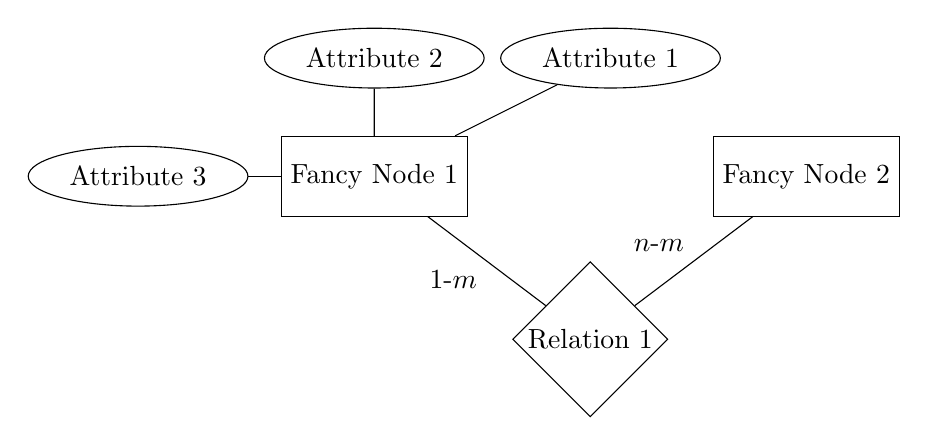
\begin{tikzpicture}[auto,node distance=1.5cm]
  \node[entity] (node1) {Fancy Node 1}
    [grow=up,sibling distance=3cm]
    child {node[attribute] {Attribute 1}}
   child {node[attribute] {Attribute 2}}
   child[grow=left,level distance=3cm] {node[attribute] {Attribute 3}};
 % Now place a relation (ID=rel1)
 \node[relationship] (rel1) [below right = of node1] {Relation 1};
 % Now the 2nd entity (ID=rel2)
 \node[entity] (node2) [above right = of rel1]	{Fancy Node 2};
 % Draw an edge between rel1 and node1; rel1 and node2
 \path (rel1) edge node {1-\(m\)} (node1)
   edge	 node {\(n\)-\(m\)}	(node2);
\end{tikzpicture}

\section{\tl{Quantum Parallelism}}

\section{\tl{Deutsch's Algorithm}}

\section{\tl{Deutsch-Jozsa Algorithm}}

\section{\tl{Simon's Algorithm}}

\section{\tl{Grover's Algorithm}}

\section{\tl{Quantum Search Algorithms}}

	\chapter{\selectlanguage{english}The quantum Fourier Transformation}

\section{\selectlanguage{english}FFT}

\section{\selectlanguage{english}QFT}

	\chapter{\tl{The Shor's Code}}

\section{\tl{Quantum error-correction}}

	\include{Chapters/RSACryptosystem}
	\chapter{\tl{Future Work/What's Happening Now}}

	\include{Chapters/Summary}
% Παραρτήματα
	\appendix
	\include{appA}
	\cleardoublepage
% Βιβλιογραφία - Αναφορές
	\bibliography{references}
% Συντομογραφίες - Αρκτικόλεξα - Ακρωνύμια
	\include{abbreviations}
% Γλωσσάριο
	\include{glossary}
%%%%%%%%%%%%%%%%%%%%%%%%%%%%%%%%%%%%%%%%%%%%%%%%%%%%
\backmatter
% Ευρετήριο Όρων
	\printindex
	\cleardoublepage

%%%%%%%%%%%%%%%%%%
%%%%%%%%%%%%%%%%%%

%% Δημιουργία ετικετών CD:

	\definecdlabeloffsets{0}{-0.65}{0}{0.55} % upper label x offset [cm] (default=0) /  upper label y offset [cm] (default=0) /  lower label x offset [cm] (default=0) /  lower  label y offset [cm] (default=0) -- For Q-Connect KF01579 labels use the following offset values: {0}{-0.65}{0}{0.55}

	\createcdlabel{Πρότυπο Σύστημα Ομότιμων \\ Κόμβων Βασισμένο σε Σχήματα \en{RDF}}{Κωνσταντίνος Δ. Δημητρίου}{ΟΚΤΩΒΡΙΟΣ}{2014}{8} % τίτλος πτυχιακής / όνομα συγγραφέα / μήνας / έτος / εύρος περιοχής τίτλου σε cm (προτεινόμενη τιμή: 8)

%%
%% Δημιουργία εξωφύλλου θήκης CD:

	\createcdcover{Πρότυπο Σύστημα Ομότιμων \\ Κόμβων Βασισμένο σε Σχήματα \en{RDF}}{Κωνσταντίνος Δ. Δημητρίου}{ΟΚΤΩΒΡΙΟΣ}{2014}{10} % τίτλος πτυχιακής / όνομα συγγραφέα / μήνας / έτος / εύρος περιοχής τίτλου σε cm (προτεινόμενη τιμή: 10)

%%%
	\pagebreak
	\thispagestyle{empty}
\end{document}
